\section{Resultados experimentales: Solomon (100 clientes)}
\label{sec:experimentos}

Esta sección presenta los resultados de los dos métodos sobre las instancias de
Solomon~\cite{solomon1987}. Todos los valores proceden de una única campaña ejecutada con la
versión del código descrita en este documento (recalentamiento solo en la fase~1,
Sección~\ref{sec:base}). Los datos crudos están en el archivo \cod{master\_solomon.csv} de
\cod{Experiments/results/solomon/} y los agregados en \cod{Experiments/summary/solomon/}.

\subsection{Diseño experimental}
\label{sec:exp-diseno}

\begin{itemize}
\item \textbf{Instancias.} Las $56$ instancias de $100$ clientes, agrupadas en seis clases:
C1 ($9$), C2 ($8$), R1 ($12$), R2 ($11$), RC1 ($8$) y RC2 ($8$). La letra indica la
distribución geográfica (agrupada, aleatoria o mixta) y el dígito el horizonte: en las clases
de tipo~1 las ventanas son estrechas y las rutas cortas (del orden de $10$ a $19$ vehículos);
en las de tipo~2 el horizonte es largo y bastan entre $2$ y $4$ vehículos.
\item \textbf{Presupuesto.} $T_{\max}=25\,000$ iteraciones, es decir, entre $25\,000$ y
$50\,000$ iteraciones por corrida según lo que consuma la fase~1. Los parámetros del
Q-learning son los valores por defecto de \cod{SolverParams}.
\item \textbf{Repeticiones.} $10$ corridas por instancia y algoritmo: $56\times 2\times 10=1120$
corridas. Las $1120$ terminaron con una solución válida (todas las rutas factibles y ningún
cliente sin asignar).
\item \textbf{Semillas pareadas.} La semilla de la corrida $k$ de una instancia es
$(12345+\mathrm{crc32}(\textit{nombre})+7919\,k)\bmod(2^{31}-1)$ y es la misma para los dos
algoritmos, de modo que ambos parten de la misma solución inicial y la comparación es pareada.
\item \textbf{Referencia.} Las mejores soluciones conocidas (BKS) son las publicadas por
SINTEF para el objetivo jerárquico (primero vehículos, después distancia), recogidas en el
archivo \cod{sintef\_solomon.csv} de \cod{Experiments/sintef/}.
\item \textbf{Ejecución.} Las corridas se lanzaron en paralelo, con $16$ procesos simultáneos
en un mismo equipo. El tiempo de CPU que se reporta está afectado por esa concurrencia y debe
leerse como orientativo y útil solo para comparar los dos métodos entre sí.
\end{itemize}

\subsection{Métricas}
\label{sec:exp-metricas}

Para cada instancia y algoritmo se promedian las $10$ corridas, lo que da un número medio de
vehículos $\mathrm{NV}$ y una distancia media $\mathrm{TD}$. A partir de ellos se usan:

\begin{itemize}
\item \textbf{Brecha por clase.} Con $\overline{\mathrm{NV}}$ y $\overline{\mathrm{TD}}$ las
medias de la clase,
\[
\mathrm{GAP}_{\mathrm{NV}}=100\,\frac{\overline{\mathrm{NV}}-\overline{\mathrm{NV}}_{\mathrm{BKS}}}{\overline{\mathrm{NV}}_{\mathrm{BKS}}},
\qquad
\mathrm{GAP}_{\mathrm{TD}}=100\,\frac{\overline{\mathrm{TD}}-\overline{\mathrm{TD}}_{\mathrm{BKS}}}{\overline{\mathrm{TD}}_{\mathrm{BKS}}}.
\]
\item \textbf{Mejora del Q-learning sobre el ALNS clásico (IMP).}
\[
\mathrm{IMP}_{\mathrm{NV}}=100\,\frac{\overline{\mathrm{NV}}_{\mathrm{ALNS}}-\overline{\mathrm{NV}}_{\mathrm{Q}}}{\overline{\mathrm{NV}}_{\mathrm{ALNS}}},
\qquad
\mathrm{IMP}_{\mathrm{TD}}=100\,\frac{\overline{\mathrm{TD}}_{\mathrm{ALNS}}-\overline{\mathrm{TD}}_{\mathrm{Q}}}{\overline{\mathrm{TD}}_{\mathrm{ALNS}}}.
\]
Un valor positivo favorece al Q-learning.
\item \textbf{Brecha de distancia auditada.} Como el objetivo es jerárquico, una distancia
solo es comparable con la del BKS si se obtuvo con su misma flota: con un vehículo de más la
distancia suele ser \emph{menor} que la del BKS, y la brecha sale negativa sin que la solución
sea mejor. Por eso la brecha de distancia por instancia se calcula únicamente en las
instancias en las que la flota media de las $10$ corridas iguala la del BKS; en el resto se
reporta solo el exceso de flota.
\item \textbf{Marcador directo.} Cada instancia se asigna al método con menor flota media y, a
igualdad de flota, al de menor distancia media (orden lexicográfico).
\item \textbf{Contraste estadístico.} Prueba de rangos con signo de Wilcoxon sobre las $56$
instancias, pareada por instancia, con nivel de significación $0.05$.
\end{itemize}

\subsection{Resultados por clase}

La Tabla~\ref{tab:sol-clases} resume los resultados. La fila global es la media de las seis
clases.

\begin{table}[H]
\centering
\small
\caption{Solomon, 100 clientes: medias por clase de las $10$ corridas (NV / TD), brecha
respecto del BKS e IMP del Q-learning sobre el ALNS clásico. Brechas e IMP en porcentaje.}
\label{tab:sol-clases}
\footnotesize
\setlength{\tabcolsep}{4.5pt}
\begin{tabular}{@{}l c c c c c c@{}}
\toprule
 & BKS & ALNS clásico & ALNS-Q & GAP ALNS & GAP ALNS-Q & IMP \\
Clase & NV / TD & NV / TD & NV / TD & NV / TD & NV / TD & NV / TD \\
\midrule
C1  & 10.00 / 828.38  & 10.00 / 828.38  & 10.00 / 828.38  & 0.00 / 0.00 & 0.00 / 0.00 & 0.00 / 0.00 \\
C2  & 3.00 / 589.86   & 3.00 / 589.86   & 3.00 / 589.86   & 0.00 / 0.00 & 0.00 / 0.00 & 0.00 / 0.00 \\
R1  & 11.92 / 1210.34 & 12.09 / 1217.11 & 12.09 / 1215.66 & 1.47 / 0.56 & 1.47 / 0.44 & 0.00 / $+0.12$ \\
R2  & 2.73 / 951.03   & 2.78 / 959.59   & 2.75 / 967.91   & 2.00 / 0.90 & 0.67 / 1.77 & $+1.31$ / $-0.87$ \\
RC1 & 11.50 / 1384.16 & 11.62 / 1388.24 & 11.65 / 1385.03 & 1.09 / 0.29 & 1.30 / 0.06 & $-0.22$ / $+0.23$ \\
RC2 & 3.25 / 1119.24  & 3.25 / 1144.28  & 3.25 / 1140.94  & 0.00 / 2.24 & 0.00 / 1.94 & 0.00 / $+0.29$ \\
\midrule
Global & 7.07 / 1013.83 & 7.12 / 1021.24 & 7.12 / 1021.30 & 0.84 / 0.73 & 0.81 / 0.74 & $+0.03$ / $-0.01$ \\
\bottomrule
\end{tabular}
\end{table}

Tres observaciones:

\begin{itemize}
\item \textbf{Clases agrupadas.} En C1 y C2 los dos métodos alcanzan el BKS, en flota y en
distancia, en las $170$ corridas de cada uno. Estas $17$ instancias no discriminan entre los
métodos.
\item \textbf{Nivel de calidad.} En las cuatro clases restantes ambos métodos quedan, en
promedio, a menos del $2$\,\% del BKS en flota y a menos del $2.3$\,\% en distancia. En el
promedio global la brecha es de $0.8$\,\% en vehículos y de $0.7$\,\% en distancia para los
dos.
\item \textbf{Diferencia entre métodos.} El IMP global es prácticamente nulo ($+0.03$\,\% en
vehículos y $-0.01$\,\% en distancia). Por clase, el Q-learning usa menos vehículos en R2 y
algo más en RC1, y obtiene menos distancia en R1, RC1 y RC2. El único IMP de distancia
negativo, el de R2, coincide con la clase en la que el Q-learning usa menos vehículos y se
explica por ello: en las nueve instancias de R2 en que ambos métodos emplean la misma flota
media, el IMP de distancia es $+0.05$\,\%.
\end{itemize}

\subsection{Minimización de flota}

La Tabla~\ref{tab:sol-flota} mide con qué frecuencia se alcanza la flota del BKS, que es el
objetivo prioritario.

\begin{table}[H]
\centering
\small
\caption{Solomon, 100 clientes: instancias cuya flota media iguala la del BKS y corridas
individuales que la igualan.}
\label{tab:sol-flota}
\begin{tabular}{@{}l c c c c c@{}}
\toprule
 & & \multicolumn{2}{c}{Instancias con flota media = BKS} & \multicolumn{2}{c}{Corridas con flota = BKS} \\
\cmidrule(lr){3-4}\cmidrule(l){5-6}
Clase & Instancias & ALNS clásico & ALNS-Q & ALNS clásico & ALNS-Q \\
\midrule
C1  & 9  & 9  & 9  & 90 / 90   & 90 / 90 \\
C2  & 8  & 8  & 8  & 80 / 80   & 80 / 80 \\
R1  & 12 & 7  & 8  & 99 / 120  & 99 / 120 \\
R2  & 11 & 8  & 9  & 104 / 110 & 108 / 110 \\
RC1 & 8  & 5  & 5  & 70 / 80   & 68 / 80 \\
RC2 & 8  & 8  & 8  & 80 / 80   & 80 / 80 \\
\midrule
Total & 56 & 45 & 47 & 523 / 560 & 525 / 560 \\
\bottomrule
\end{tabular}
\end{table}

El ALNS clásico iguala la flota del BKS en el $93.4$\,\% de las corridas y el Q-learning en
el $93.8$\,\%. Considerando la mejor de las $10$ corridas, \emph{los dos métodos alcanzan la
flota del BKS en las $56$ instancias}; ninguno la mejora. Las corridas con un vehículo de más
se concentran en $11$ instancias de R1, R2 y RC1 (Tabla~\ref{tab:sol-exceso}), que son las
mismas para ambos métodos salvo R111 y R202, en las que el Q-learning iguala al BKS en las
diez corridas. La diferencia de flota entre métodos
no es estadísticamente significativa (Wilcoxon, $p=0.75$). Por corrida, con la misma semilla,
el Q-learning usa menos vehículos en $15$ de los $560$ pares, el clásico en $13$ y coinciden
en $532$.

\begin{table}[H]
\centering
\small
\caption{Instancias en las que algún método no iguala la flota del BKS en las $10$ corridas:
flota media de cada método.}
\label{tab:sol-exceso}
\begin{tabular}{@{}l c c c @{\hspace{2.5em}} l c c c@{}}
\toprule
Instancia & BKS & ALNS & ALNS-Q & Instancia & BKS & ALNS & ALNS-Q \\
\midrule
R104 & 9  & 9.9  & 9.8  & R207  & 2  & 2.1  & 2.1 \\
R109 & 11 & 11.2 & 11.2 & R211  & 2  & 2.4  & 2.1 \\
R110 & 10 & 10.2 & 10.2 & RC102 & 12 & 12.2 & 12.2 \\
R111 & 10 & 10.1 & 10.0 & RC105 & 13 & 13.1 & 13.3 \\
R112 & 9  & 9.7  & 9.9  & RC106 & 11 & 11.7 & 11.7 \\
R202 & 3  & 3.1  & 3.0  &       &    &      &     \\
\bottomrule
\end{tabular}
\end{table}

Las instancias más difíciles en flota son R104, R112 y RC106, en las que el vehículo
adicional aparece en la mayoría de las corridas de los dos métodos: en ellas la fase~1
(Sección~\ref{sec:fases}) rara vez consigue vaciar el banco de la última ruta eliminada.

\subsection{Calidad de ruta}

La Tabla~\ref{tab:sol-gap} recoge la brecha de distancia auditada. Para comparar los métodos
sobre el mismo conjunto, se añade la brecha restringida a las $45$ instancias en las que
\emph{ambos} igualan la flota del BKS, y la brecha de la mejor de las $10$ corridas, que está
definida en las $56$ instancias porque la mejor corrida siempre iguala la flota del BKS.

\begin{table}[H]
\centering
\small
\caption{Solomon, 100 clientes: brecha de distancia respecto del BKS, en porcentaje. Entre
paréntesis, número de instancias sobre el que se promedia.}
\label{tab:sol-gap}
\begin{tabular}{@{}l c c c c c c c@{}}
\toprule
 & \multicolumn{2}{c}{Media, auditada} & \multicolumn{3}{c}{Media, instancias comunes} & \multicolumn{2}{c}{Mejor de $10$} \\
\cmidrule(lr){2-3}\cmidrule(lr){4-6}\cmidrule(l){7-8}
Clase & ALNS & ALNS-Q & $n$ & ALNS & ALNS-Q & ALNS & ALNS-Q \\
\midrule
C1  & 0.00 (9) & 0.00 (9) & 9 & 0.00 & 0.00 & 0.00 & 0.00 \\
C2  & 0.00 (8) & 0.00 (8) & 8 & 0.00 & 0.00 & 0.00 & 0.00 \\
R1  & 0.56 (7) & 0.50 (8) & 7 & 0.56 & 0.40 & 0.47 & 0.42 \\
R2  & 1.23 (8) & 1.50 (9) & 8 & 1.23 & 1.29 & 0.35 & 0.46 \\
RC1 & 1.02 (5) & 0.88 (5) & 5 & 1.02 & 0.88 & 0.09 & 0.17 \\
RC2 & 2.07 (8) & 1.76 (8) & 8 & 2.07 & 1.76 & 0.49 & 0.15 \\
\midrule
Total & 0.79 (45) & 0.77 (47) & 45 & 0.79 & 0.70 & 0.25 & 0.23 \\
\bottomrule
\end{tabular}
\end{table}

En las $45$ instancias comunes la brecha media del Q-learning es $0.70$\,\% frente a
$0.79$\,\% del ALNS clásico; es menor en R1, RC1 y RC2 y mayor en R2. La diferencia no es
estadísticamente significativa (Wilcoxon, $n=45$, $p=0.23$). La mejor de las $10$ corridas
queda a $0.25$\,\% y $0.23$\,\% del BKS, respectivamente, con la flota del BKS en todas las
instancias. La distancia entre la brecha media y la de la mejor corrida, que es mayor en las
clases de horizonte largo (R2 y RC2), indica que en ellas el resultado depende más de la
semilla.

La comparación directa entre métodos, sin pasar por el BKS, usa las $50$ instancias en las
que ambos obtienen la misma flota media. En ellas el IMP medio de distancia es $+0.10$\,\%
($+0.15$\,\% en R1, $+0.05$\,\% en R2, $+0.10$\,\% en RC1 y $+0.30$\,\% en RC2): el Q-learning
obtiene menos distancia en $19$ instancias, el clásico en $14$ y empatan en $17$. Tampoco esta
diferencia es significativa (Wilcoxon, $p=0.24$). Por corrida, en los $532$ pares con la
misma flota el Q-learning obtiene menos distancia en $167$, el clásico en $152$ y coinciden
en $213$.

\subsection{Marcador directo y tiempo de cómputo}

\begin{table}[H]
\centering
\small
\caption{Solomon, 100 clientes: marcador lexicográfico del Q-learning frente al ALNS clásico
(instancias ganadas, empatadas y perdidas) y tiempo medio de CPU por corrida, en segundos.}
\label{tab:sol-marcador}
\begin{tabular}{@{}l c c c c c@{}}
\toprule
 & \multicolumn{3}{c}{ALNS-Q frente a ALNS} & \multicolumn{2}{c}{Tiempo de CPU (s)} \\
\cmidrule(lr){2-4}\cmidrule(l){5-6}
Clase & Gana & Empata & Pierde & ALNS clásico & ALNS-Q \\
\midrule
C1  & 0 & 9 & 0 & 2.44 & 2.52 \\
C2  & 0 & 8 & 0 & 3.89 & 4.03 \\
R1  & 7 & 0 & 5 & 5.08 & 4.55 \\
R2  & 6 & 0 & 5 & 6.64 & 6.75 \\
RC1 & 4 & 0 & 4 & 4.32 & 4.81 \\
RC2 & 6 & 0 & 2 & 6.53 & 5.96 \\
\midrule
Total & 23 & 17 & 16 & 4.89 & 4.82 \\
\bottomrule
\end{tabular}
\end{table}

El Q-learning gana $23$ instancias, pierde $16$ y empata $17$ (las de C1 y C2). Fuera de las
clases agrupadas el marcador es $23$ a $16$, con la ventaja más clara en RC2. El costo
computacional es equivalente: $4.89$~s y $4.82$~s por corrida en promedio, sin diferencia
significativa (Wilcoxon, $p=0.96$). Esto es coherente con el diseño: los dos métodos ejecutan
los mismos operadores y solo difieren en la selección y el aprendizaje, cuyo costo es
despreciable frente al de la reparación (Sección~\ref{sec:reparacion}). Las clases de
horizonte largo (R2 y RC2), con rutas más largas, son las más costosas para ambos.

\subsection{Distribución por corrida}

Las Figuras~\ref{fig:sol-box-veh} y~\ref{fig:sol-box-dist} muestran la distribución de la
brecha de cada corrida individual, sin auditar. En vehículos, las cajas están colapsadas en
cero y los puntos aislados corresponden a las corridas con un vehículo de más; como las clases
de tipo~2 usan dos o tres vehículos, un solo vehículo adicional supone allí una brecha del
$33$\,\% o del $50$\,\%. En distancia, los valores negativos son precisamente esas corridas:
usan más vehículos que el BKS y por eso recorren menos. La
Figura~\ref{fig:sol-scatter} compara, instancia a instancia, la brecha media de distancia de
los dos métodos: los puntos se disponen a ambos lados de la diagonal sin un sesgo apreciable.

\begin{figure}[H]
\centering
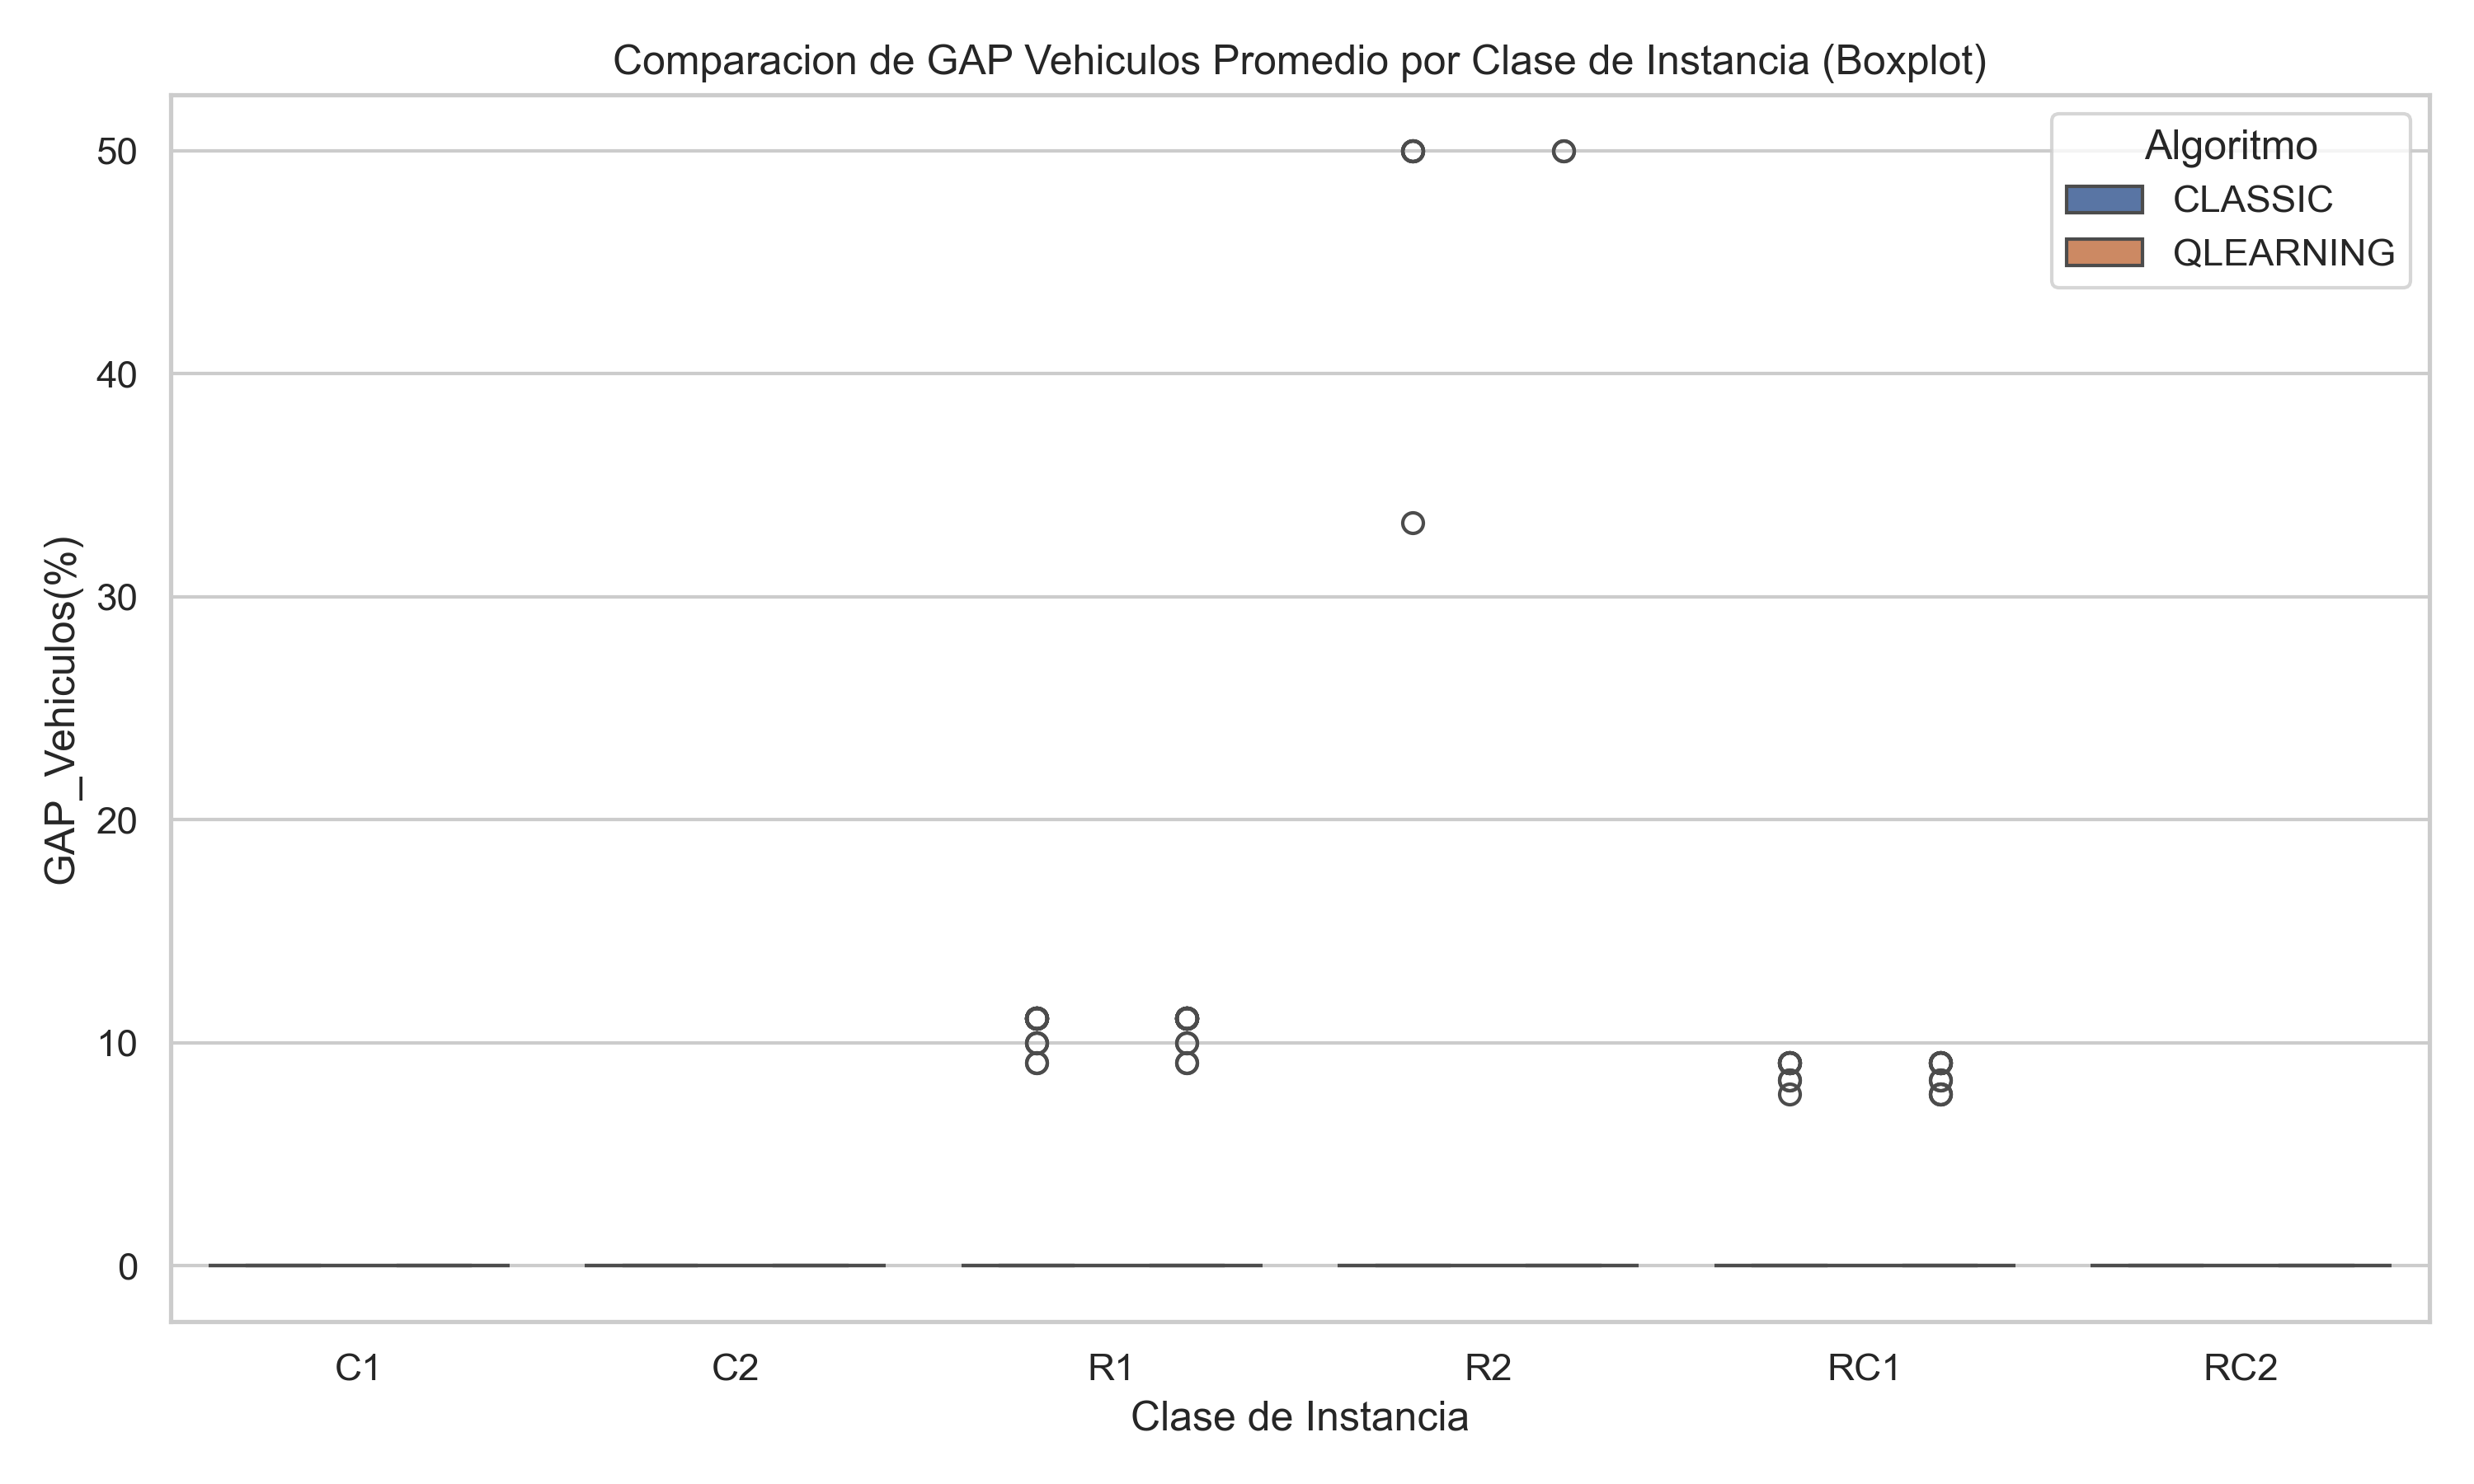
\includegraphics[width=0.78\textwidth]{../Experiments/figs/solomon/boxplot_gap_vehiculos.png}
\caption{Brecha de vehículos por corrida respecto del BKS, por clase.}
\label{fig:sol-box-veh}
\end{figure}

\begin{figure}[H]
\centering
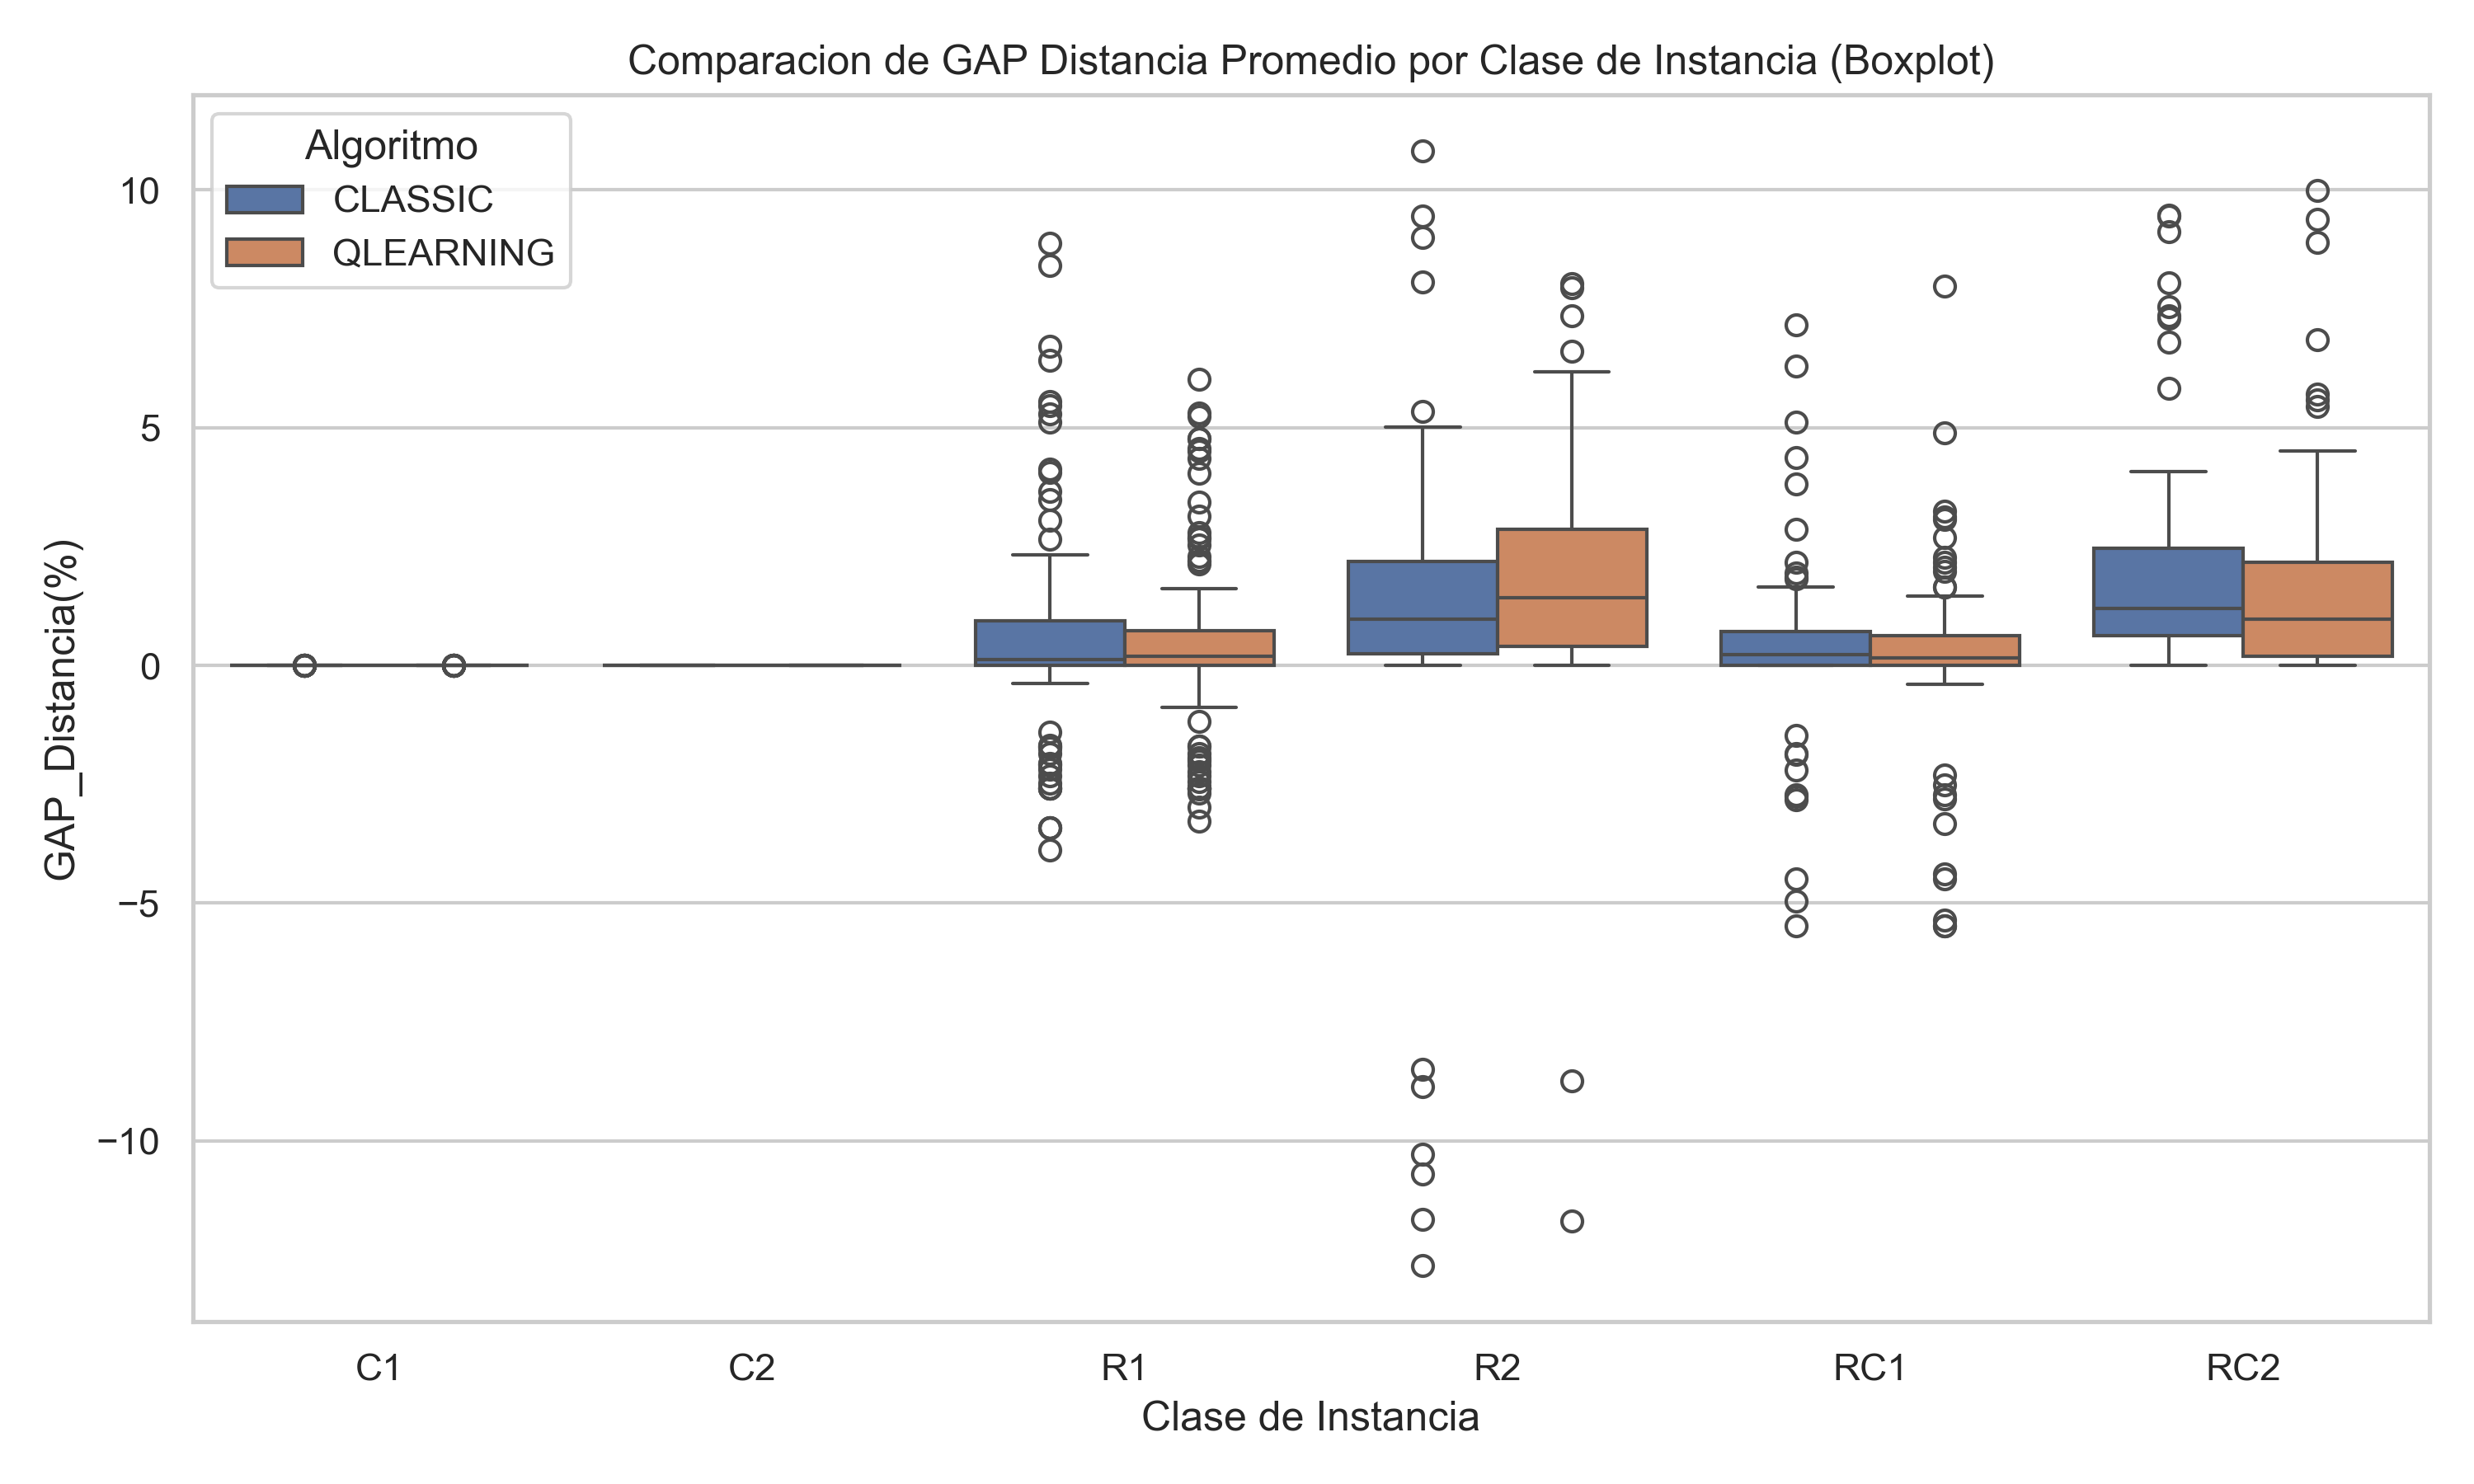
\includegraphics[width=0.78\textwidth]{../Experiments/figs/solomon/boxplot_gap_distancia.png}
\caption{Brecha de distancia por corrida respecto del BKS, por clase (sin auditar: los
valores negativos son corridas con más vehículos que el BKS).}
\label{fig:sol-box-dist}
\end{figure}

\begin{figure}[H]
\centering
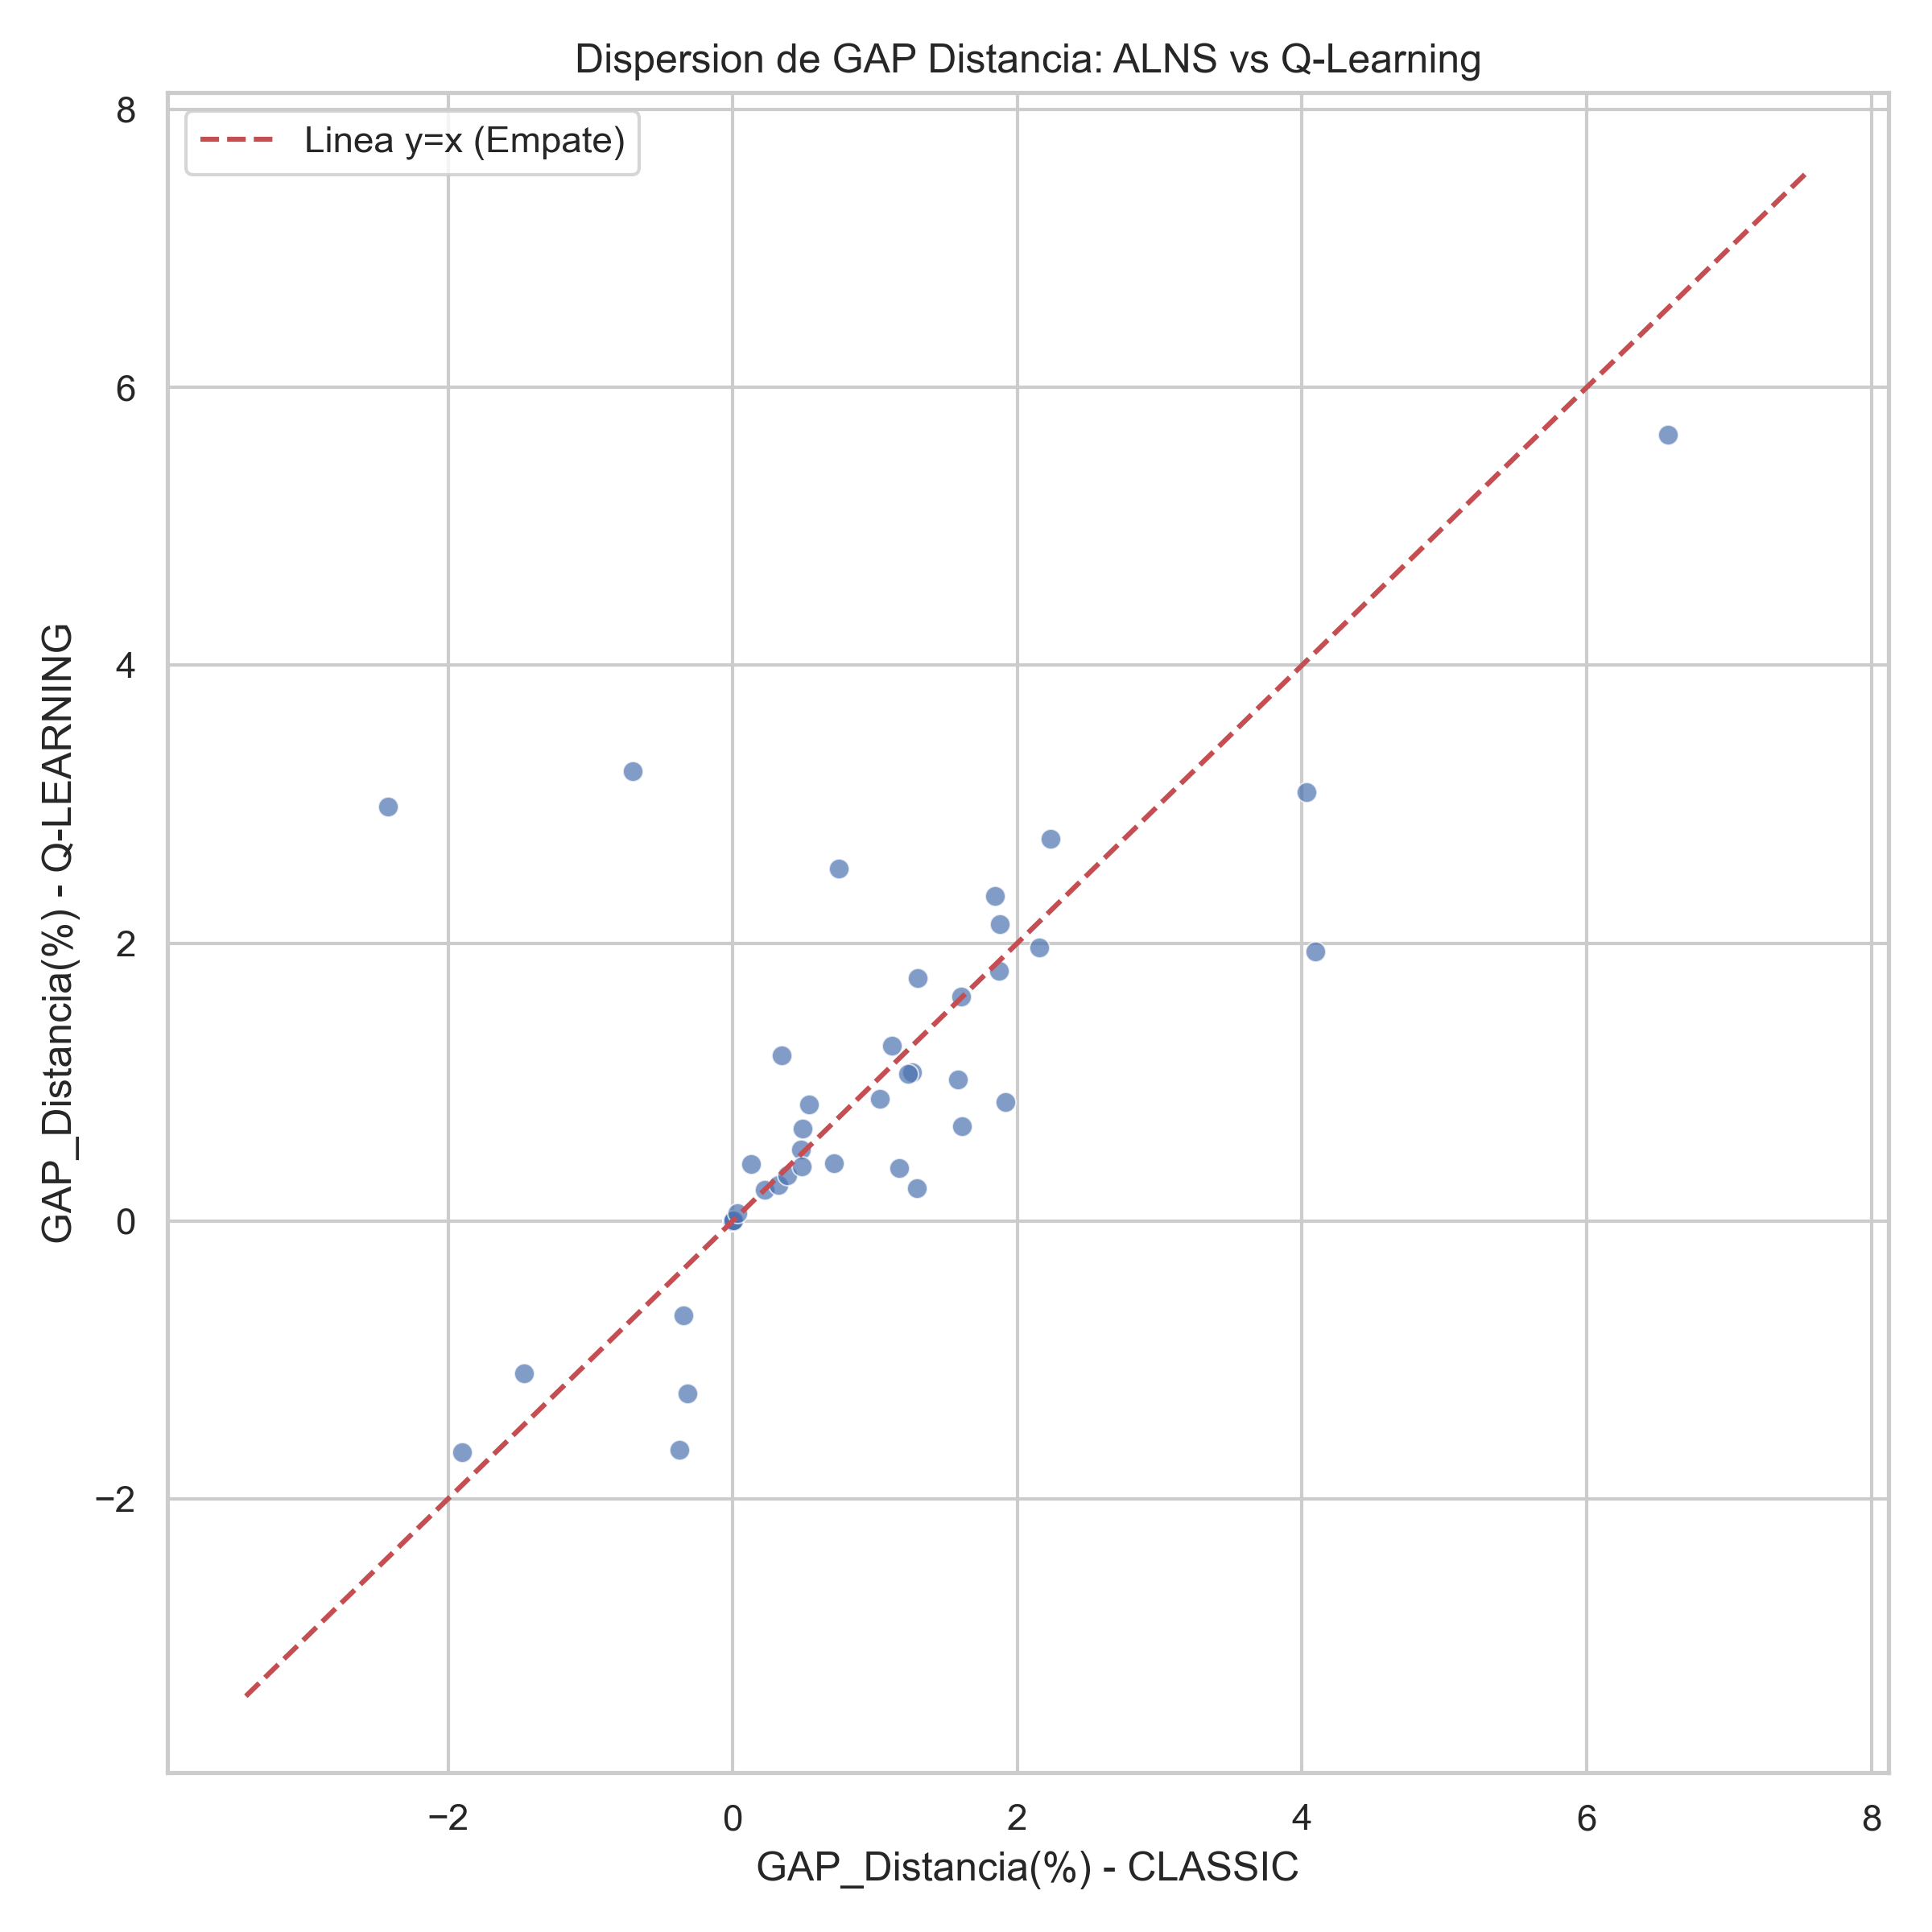
\includegraphics[width=0.6\textwidth]{../Experiments/figs/solomon/scatter_gap_distancia.png}
\caption{Brecha media de distancia por instancia: ALNS clásico (abscisas) frente a
Q-learning (ordenadas). Por debajo de la diagonal el Q-learning es mejor.}
\label{fig:sol-scatter}
\end{figure}

\subsection{Discusión}
\label{sec:exp-discusion}

\begin{itemize}
\item \textbf{Ambos métodos son competitivos en este tamaño.} Con $25\,000$ iteraciones de
fase~2 y unos $5$ segundos por corrida, los dos alcanzan la flota del BKS en todas las
instancias en al menos una de las diez corridas, y en el $93$\,\% de las corridas
individuales; la mejor corrida queda a un cuarto de punto porcentual del BKS en distancia.
Este nivel se debe a los componentes comunes (Sección~\ref{sec:sintesis}): la fase propia de
reducción de flota, el catálogo de operadores y el esquema de temperatura.
\item \textbf{No hay diferencia significativa entre los mecanismos de selección.} El
Q-learning queda ligeramente por delante en casi todos los indicadores agregados (marcador
$23$ a $16$, brecha en instancias comunes $0.70$\,\% frente a $0.79$\,\%, dos instancias más
con la flota del BKS), pero ninguna de las pruebas alcanza significación y la magnitud de las
diferencias, del orden de una décima de punto porcentual, es inferior a la variación entre
semillas. Con estos datos no puede afirmarse que un método supere al otro en instancias de
$100$ clientes.
\item \textbf{Dónde aparece la diferencia.} Las diferencias, cuando las hay, se concentran en
las clases con clientes dispersos y son nulas en las agrupadas. En R2 el Q-learning reduce
flota (iguala al BKS en $108$ de $110$ corridas, frente a $104$) a costa de distancia; en RC2,
con flota idéntica, reduce la brecha de $2.07$\,\% a $1.76$\,\%; en RC1 el clásico iguala la
flota del BKS en dos corridas más.
\item \textbf{Efecto techo.} Diecisiete de las $56$ instancias las resuelven ambos métodos en
todas las corridas, y en la mayoría de las restantes el margen respecto del BKS es inferior
al $2$\,\%. Con tan poco margen de mejora, este conjunto discrimina mal entre mecanismos de
selección: el presupuesto de iteraciones basta para que una selección menos informada llegue
a soluciones de calidad similar. Las diferencias de mecanismo descritas en la
Sección~\ref{sec:sintesis} deberían manifestarse con más claridad cuando el presupuesto es
escaso en relación con el tamaño de la instancia, lo que corresponde a las instancias de
Gehring y Homberger~\cite{gehring1999}, cuyos resultados no se incluyen en esta sección.
\end{itemize}

\subsection{Resultados por instancia}

Las Tablas~\ref{tab:sol-instancias} y~\ref{tab:sol-instancias-b} detallan las $56$ instancias. Las columnas NV y TD son medias
de las $10$ corridas; GAP es la brecha de distancia auditada, en porcentaje, y se omite (--)
cuando la flota media supera la del BKS; la mejor corrida es la mejor de las $10$ en orden
lexicográfico, expresada como vehículos/distancia.

\begin{table}[H]
\centering
\footnotesize
\setlength{\tabcolsep}{4pt}
\caption{Solomon, 100 clientes: resultados por instancia, clases C1, C2 y R1.}
\label{tab:sol-instancias}
\begin{tabular}{@{}l r r r r r r r r r r@{}}
\toprule
 & \multicolumn{2}{c}{BKS} & \multicolumn{3}{c}{ALNS clásico (media)} & \multicolumn{3}{c}{ALNS-Q (media)} & \multicolumn{2}{c}{Mejor corrida} \\
\cmidrule(lr){2-3}\cmidrule(lr){4-6}\cmidrule(lr){7-9}\cmidrule(l){10-11}
Inst. & NV & TD & NV & TD & GAP & NV & TD & GAP & ALNS & ALNS-Q \\
\midrule
% Filas generadas desde Experiments/results/solomon/master_solomon.csv
C101 & 10 & 828.94 & 10.0 & 828.94 & 0.00 & 10.0 & 828.94 & 0.00 & 10/828.94 & 10/828.94 \\
C102 & 10 & 828.94 & 10.0 & 828.94 & 0.00 & 10.0 & 828.94 & 0.00 & 10/828.94 & 10/828.94 \\
C103 & 10 & 828.06 & 10.0 & 828.07 & 0.00 & 10.0 & 828.07 & 0.00 & 10/828.07 & 10/828.07 \\
C104 & 10 & 824.78 & 10.0 & 824.78 & 0.00 & 10.0 & 824.78 & 0.00 & 10/824.78 & 10/824.78 \\
C105 & 10 & 828.94 & 10.0 & 828.94 & 0.00 & 10.0 & 828.94 & 0.00 & 10/828.94 & 10/828.94 \\
C106 & 10 & 828.94 & 10.0 & 828.94 & 0.00 & 10.0 & 828.94 & 0.00 & 10/828.94 & 10/828.94 \\
C107 & 10 & 828.94 & 10.0 & 828.94 & 0.00 & 10.0 & 828.94 & 0.00 & 10/828.94 & 10/828.94 \\
C108 & 10 & 828.94 & 10.0 & 828.94 & 0.00 & 10.0 & 828.94 & 0.00 & 10/828.94 & 10/828.94 \\
C109 & 10 & 828.94 & 10.0 & 828.94 & 0.00 & 10.0 & 828.94 & 0.00 & 10/828.94 & 10/828.94 \\
\addlinespace
C201 & 3 & 591.56 & 3.0 & 591.56 & 0.00 & 3.0 & 591.56 & 0.00 & 3/591.56 & 3/591.56 \\
C202 & 3 & 591.56 & 3.0 & 591.56 & 0.00 & 3.0 & 591.56 & 0.00 & 3/591.56 & 3/591.56 \\
C203 & 3 & 591.17 & 3.0 & 591.17 & 0.00 & 3.0 & 591.17 & 0.00 & 3/591.17 & 3/591.17 \\
C204 & 3 & 590.60 & 3.0 & 590.60 & 0.00 & 3.0 & 590.60 & 0.00 & 3/590.60 & 3/590.60 \\
C205 & 3 & 588.88 & 3.0 & 588.88 & 0.00 & 3.0 & 588.88 & 0.00 & 3/588.88 & 3/588.88 \\
C206 & 3 & 588.49 & 3.0 & 588.49 & 0.00 & 3.0 & 588.49 & 0.00 & 3/588.49 & 3/588.49 \\
C207 & 3 & 588.29 & 3.0 & 588.29 & 0.00 & 3.0 & 588.29 & 0.00 & 3/588.29 & 3/588.29 \\
C208 & 3 & 588.32 & 3.0 & 588.32 & 0.00 & 3.0 & 588.32 & 0.00 & 3/588.32 & 3/588.32 \\
\addlinespace
R101 & 19 & 1650.80 & 19.0 & 1650.85 & 0.00 & 19.0 & 1650.88 & 0.00 & 19/1650.80 & 19/1650.80 \\
R102 & 17 & 1486.12 & 17.0 & 1486.59 & 0.03 & 17.0 & 1486.95 & 0.06 & 17/1486.12 & 17/1486.12 \\
R103 & 13 & 1292.68 & 13.0 & 1295.62 & 0.23 & 13.0 & 1295.56 & 0.22 & 13/1292.68 & 13/1292.68 \\
R104 & 9 & 1007.31 & 9.9 & 988.14 & -- & 9.8 & 990.54 & -- & 9/1007.31 & 9/1007.31 \\
R105 & 14 & 1377.11 & 14.0 & 1381.53 & 0.32 & 14.0 & 1380.66 & 0.26 & 14/1377.11 & 14/1377.11 \\
R106 & 12 & 1252.03 & 12.0 & 1258.00 & 0.48 & 12.0 & 1258.45 & 0.51 & 12/1252.03 & 12/1252.03 \\
R107 & 10 & 1104.66 & 10.0 & 1118.58 & 1.26 & 10.0 & 1116.51 & 1.07 & 10/1111.44 & 10/1104.66 \\
R108 & 9 & 960.88 & 9.0 & 976.33 & 1.61 & 9.0 & 967.45 & 0.68 & 9/963.66 & 9/960.88 \\
R109 & 11 & 1194.73 & 11.2 & 1243.62 & -- & 11.2 & 1217.93 & -- & 11/1226.49 & 11/1201.41 \\
R110 & 10 & 1118.84 & 10.2 & 1127.15 & -- & 10.2 & 1147.20 & -- & 10/1118.84 & 10/1142.75 \\
R111 & 10 & 1096.73 & 10.1 & 1100.49 & -- & 10.0 & 1109.79 & 1.19 & 10/1096.73 & 10/1096.73 \\
R112 & 9 & 982.14 & 9.7 & 978.45 & -- & 9.9 & 965.98 & -- & 9/1002.26 & 9/1004.60 \\
\bottomrule
\end{tabular}
\end{table}

\begin{table}[H]
\centering
\footnotesize
\setlength{\tabcolsep}{4pt}
\caption{Solomon, 100 clientes: resultados por instancia, clases R2, RC1 y RC2.}
\label{tab:sol-instancias-b}
\begin{tabular}{@{}l r r r r r r r r r r@{}}
\toprule
 & \multicolumn{2}{c}{BKS} & \multicolumn{3}{c}{ALNS clásico (media)} & \multicolumn{3}{c}{ALNS-Q (media)} & \multicolumn{2}{c}{Mejor corrida} \\
\cmidrule(lr){2-3}\cmidrule(lr){4-6}\cmidrule(lr){7-9}\cmidrule(l){10-11}
Inst. & NV & TD & NV & TD & GAP & NV & TD & GAP & ALNS & ALNS-Q \\
\midrule
% Filas generadas desde Experiments/results/solomon/master_solomon.csv
R201 & 4 & 1252.37 & 4.0 & 1253.98 & 0.13 & 4.0 & 1257.49 & 0.41 & 4/1252.37 & 4/1253.23 \\
R202 & 3 & 1191.70 & 3.1 & 1183.33 & -- & 3.0 & 1230.30 & 3.24 & 3/1191.70 & 3/1195.30 \\
R203 & 3 & 939.50 & 3.0 & 944.52 & 0.53 & 3.0 & 947.38 & 0.84 & 3/939.50 & 3/941.41 \\
R204 & 2 & 825.52 & 2.0 & 840.99 & 1.87 & 2.0 & 843.15 & 2.14 & 2/828.78 & 2/828.78 \\
R205 & 3 & 994.43 & 3.0 & 1006.70 & 1.23 & 3.0 & 1004.94 & 1.06 & 3/994.43 & 3/994.43 \\
R206 & 3 & 906.14 & 3.0 & 920.47 & 1.58 & 3.0 & 915.34 & 1.02 & 3/906.14 & 3/906.14 \\
R207 & 2 & 890.61 & 2.1 & 926.53 & -- & 2.1 & 918.08 & -- & 2/897.06 & 2/907.69 \\
R208 & 2 & 726.82 & 2.0 & 734.33 & 1.03 & 2.0 & 733.22 & 0.88 & 2/726.82 & 2/726.82 \\
R209 & 3 & 909.16 & 3.0 & 925.92 & 1.84 & 3.0 & 930.44 & 2.34 & 3/915.24 & 3/913.77 \\
R210 & 3 & 939.37 & 3.0 & 954.42 & 1.60 & 3.0 & 954.53 & 1.61 & 3/942.11 & 3/939.37 \\
R211 & 2 & 885.71 & 2.4 & 864.27 & -- & 2.1 & 912.11 & -- & 2/901.52 & 2/900.35 \\
\addlinespace
RC101 & 14 & 1696.95 & 14.0 & 1709.01 & 0.71 & 14.0 & 1703.96 & 0.41 & 14/1697.43 & 14/1696.95 \\
RC102 & 12 & 1554.75 & 12.2 & 1549.34 & -- & 12.2 & 1544.15 & -- & 12/1554.75 & 12/1554.75 \\
RC103 & 11 & 1261.67 & 11.0 & 1267.85 & 0.49 & 11.0 & 1270.07 & 0.67 & 11/1262.02 & 11/1263.54 \\
RC104 & 10 & 1135.48 & 10.0 & 1139.86 & 0.39 & 10.0 & 1139.22 & 0.33 & 10/1135.52 & 10/1135.48 \\
RC105 & 13 & 1629.44 & 13.1 & 1624.30 & -- & 13.3 & 1609.16 & -- & 13/1629.44 & 13/1629.44 \\
RC106 & 11 & 1424.73 & 11.7 & 1403.86 & -- & 11.7 & 1409.11 & -- & 11/1424.73 & 11/1432.12 \\
RC107 & 11 & 1230.48 & 11.0 & 1246.42 & 1.30 & 11.0 & 1233.41 & 0.24 & 11/1231.53 & 11/1231.53 \\
RC108 & 10 & 1139.82 & 10.0 & 1165.29 & 2.23 & 10.0 & 1171.18 & 2.75 & 10/1146.66 & 10/1146.66 \\
\addlinespace
RC201 & 4 & 1406.94 & 4.0 & 1422.65 & 1.12 & 4.0 & 1424.72 & 1.26 & 4/1415.00 & 4/1412.45 \\
RC202 & 3 & 1365.65 & 3.0 & 1455.38 & 6.57 & 3.0 & 1442.93 & 5.66 & 3/1368.04 & 3/1365.65 \\
RC203 & 3 & 1049.62 & 3.0 & 1069.28 & 1.87 & 3.0 & 1068.53 & 1.80 & 3/1061.13 & 3/1051.82 \\
RC204 & 3 & 798.46 & 3.0 & 802.33 & 0.48 & 3.0 & 801.60 & 0.39 & 3/798.46 & 3/798.46 \\
RC205 & 4 & 1297.65 & 4.0 & 1314.51 & 1.30 & 4.0 & 1320.32 & 1.75 & 4/1303.37 & 4/1302.42 \\
RC206 & 3 & 1146.32 & 3.0 & 1168.31 & 1.92 & 3.0 & 1156.15 & 0.86 & 3/1152.03 & 3/1146.32 \\
RC207 & 3 & 1061.14 & 3.0 & 1083.97 & 2.15 & 3.0 & 1082.00 & 1.97 & 3/1070.85 & 3/1061.84 \\
RC208 & 3 & 828.14 & 3.0 & 837.82 & 1.17 & 3.0 & 831.28 & 0.38 & 3/829.70 & 3/829.70 \\
\bottomrule
\end{tabular}
\end{table}
